\documentclass[12pt,a4paper]{article}
\usepackage[a4paper,margin=2cm]{geometry}
\usepackage{graphicx}
% \usepackage{minted}
\usepackage{dirtytalk}
\usepackage[T1]{fontenc}
\usepackage[math]{iwona}
\usepackage[colorlinks=true,urlcolor=blue]{hyperref}
\usepackage{helvet}
\renewcommand*{\familydefault}{\sfdefault}
\begin{document}
\title{MPHYG001: Assignment 2 \\ Bad Boids Refactoring}
\author{Padraic Calpin \\ PHDCA33}
\date{}
\maketitle

\section*{Code Smells}
\begin{description}
    \item[One Large File] \hfill \\
    The initial version of the code was a single file, which contained the initialisation,update and animation routines which could be run directly. My \href{https://github.com/padraic-padraic/bad-boids/commit/17cbde9dd7f2d8dd756ac43fcf11577f34c0b754}{initial commit}(17cbde9) defined a \texttt{Flock} class, combing the init and update routines, and the animation routines were added in commit \href{https://github.com/padraic-padraic/bad-boids/commit/7dfd3d25a5b6de1802cb93cca317e5fb79a3af8f}{7dfd3d2}. This modularisation also enabled adding a \href{https://github.com/padraic-padraic/bad-boids/commit/281e361395665c5bfad25a8b719d4190dd13c77a}{command line entry\-point}(281e361) and \href{https://github.com/padraic-padraic/bad-boids/commit/e68acc89a2c399cb0831ca96b72e49037bb61c66}{packaging the program}(e68acc8).
    \item[Loop Indexing \& Repetition] \hfill \\
    The initial code had several smells relating to the use of loops. Firstly, loops were integer indexed, and used that integer to access corresponding elements of different arrays. The same nested loop structure was also repeated four times; twice to perform the `move to middle' correction for x and y, and twice more to calculate the other velocity corrections.\\
    This was resolved by combining the positions and velocities into $2\times N \times N$ numpy arrays, and performing calculations simultaneously using broadcasting  (\href{https://github.com/padraic-padraic/bad-boids/commit/d9e6783944c37458441bec59bca9e4b98d243345}{d9e6783},\\ \href{https://github.com/padraic-padraic/bad-boids/commit/d9dfcd71929bb125dd9353619b0fc9912ddc7ac6}{d9dfcd7}, \href{https://github.com/padraic-padraic/bad-boids/commit/4a5811e5a2377f76cacd545c37c7808f1908a94b}{4a5811e},
    \href{https://github.com/padraic-padraic/bad-boids/commit/90a365990fd206db85537bc58c9a239e8dc4681a}{90a3659}).
    \item[Repeated Code]
    The initial code, and my initial refactoring to numpy arrays, contained repeated calls for x and y corrections. This was amended in commit \href{https://github.com/padraic-padraic/bad-boids/commit/90a365990fd206db85537bc58c9a239e8dc4681a}{90a3659}.
    \item[Large Routines] \hfill \\
    The \texttt{update\_boids} function, even after replacing loops with numpy broadcasting, was the bulk of the \texttt{Flock} class definition. Each component of the velocity corrections was \href{https://github.com/padraic-padraic/bad-boids/commit/cef9415816bd786d082225aec7049b268067c6f4}{split into a separate method}, which were then called sequentially in the new \texttt{update\_boids}.
    \item[Magic Numbers \& Hardcoded Constants] \hfill \\
    The initial code contained multiple hardcoded constants acting as magic numbers. The new \texttt{Flock} class loads these parameters from a descriptive config file, with the initial hardcoded values loaded as defaults (\href{https://github.com/padraic-padraic/bad-boids/commit/15dc7ae43b8428ce7197e6ccbde28344f478fc05}{15dc7ae}).
    \item[Global Variables] \hfill \\
    The animation and boid initialisation employed global variables in the initial code. I also initially made some magic numbers into global variables. These were made into properties of the \texttt{Flock} class in commits \href{https://github.com/padraic-padraic/bad-boids/commit/17cbde9dd7f2d8dd756ac43fcf11577f34c0b754}{17cbde9} and  \href{https://github.com/padraic-padraic/bad-boids/commit/7dfd3d25a5b6de1802cb93cca317e5fb79a3af8f}{7dfd3d2}
    \item[Documentation Needed] \hfill \\
    The update and animation methods were previously slightly cryptic. Turning the simulation parameters into properties of the \texttt{Flock} class(\href{https://github.com/padraic-padraic/bad-boids/commit/17cbde9dd7f2d8dd756ac43fcf11577f34c0b754}{17cbde9},\href{https://github.com/padraic-padraic/bad-boids/commit/7dfd3d25a5b6de1802cb93cca317e5fb79a3af8f}{7dfd3d2}, \href{https://github.com/padraic-padraic/bad-boids/commit/15dc7ae43b8428ce7197e6ccbde28344f478fc05}{15dc7ae}), and breaking up the update and animation functions into sub-routines (\href{https://github.com/padraic-padraic/bad-boids/commit/cef9415816bd786d082225aec7049b268067c6f4}{cef9415}), helped to make this code self-documenting. Additional docstrings were added to explain the config and data structures the Constructor expects.
    \item[Reinventing the wheel] \hfill \\
    Some components of the \texttt{update\_boids} function and the \texttt{Flock} constructor were simplified using sum, mean and random.uniform functions provided by the numpy library (\href{https://github.com/padraic-padraic/bad-boids/commit/d9e6783944c37458441bec59bca9e4b98d243345}{d9e6783}, \href{https://github.com/padraic-padraic/bad-boids/commit/d9dfcd71929bb125dd9353619b0fc9912ddc7ac6}{d9dfcd7}, \href{https://github.com/padraic-padraic/bad-boids/commit/4a5811e5a2377f76cacd545c37c7808f1908a94b}{4a5811e}, \href{https://github.com/padraic-padraic/bad-boids/commit/f090cbf5c5810bdb0068396e760e3cdbbe13a71a}{f090cbf}).


\end{description}
\section*{Class Structure}

\begin{figure}[h]
    \centering
    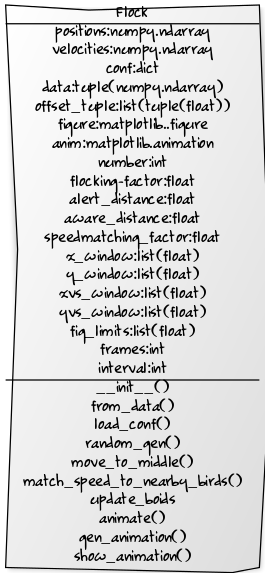
\includegraphics[width=.4\textwidth]{yUML.png}
    \caption{UML Diagram of the \texttt{Flock} class. Properties conf, data and offset\_tuple are calculated properties}
\end{figure}

\section*{The Refactoring Approach}
I think the refactoring approach is especially useful for quick translation of ideas into implementation, as might be required in an Agile development sprint, or when working to develop a `Minimally Viable' version of the code. The addition of regression tests combined with Continuous Integration then allows the code to be updated safely in production, without changing the results.

One disadvantage could be that this encourages `sloppy' design, based on the premise that it can be later refactored. There is also the possibility that regression tests allow incorrect results to propagate forward through versions, and so they cannot be used blindly; indeed, this package required a change to the regression test when refactoring altered how `speed-matching' calculation was performed.

\section*{Problems Encountered}
Already discussed above, at one point during the refactoring the regression test for \texttt{update\_boids} failed. This was because of how the previous version calculated the `speed-matching' corrections; each correction depended on the velocities of the other birds. However, as these were calculated sequentially, the corrections applied to velocities at the beginning of the list altered the calculation for birds later in the list.

When the calculation was changed to calculate all the velocity corrections simultaneously, using broadcasting, this error was corrected, but the regression test no-longer passed. This required the fixture data to be re-recorded. The change, $\mathcal{O}(0.01)$, but demonstrated the drawbacks of regression testing.

Another issue encountered was the difficulty of creating a fast, object-oriented design. In the end, I chose to optimise this code for speed, and thus there is only a single class \texttt{Flock}. A more object oriented approach might include a \texttt{Boid} class, storing the positions and velocities, which each belong to a \texttt{Flock} instance. The \texttt{Flock} could then calculate corrections by iterating over the \texttt{Boid} instances.

However, as numpy cannot create arrays of arbitrary objects, this code would be unable to take advantage of broadcasting. This could be achieved by copying the data from each boid into arrays, and then copying the updated values back into each \texttt{Boid}, but this approach is functionally the same as my \texttt{Flock} implementation.

\end{document}
